\documentclass[tikz,border=6pt]{standalone}
\usetikzlibrary{calc}

\begin{document}
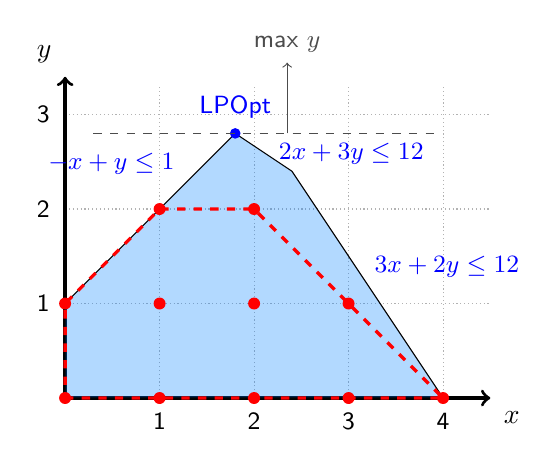
\begin{tikzpicture}[scale=1.2, every node/.style={font=\sffamily}]
  % grid
  \draw[gray!60, densely dotted, step=1] (0,0) grid (4.5,3.3);

  % axes
  \draw[very thick,->] (0,0) -- (4.5,0) node[below right=1pt] {$x$};
  \draw[very thick,->] (0,0) -- (0,3.4) node[above left=1pt] {$y$};

  % tick labels
  \foreach \x in {1,2,3,4}
    \draw (\x,0) node[below=2pt] {\small \x};
  \foreach \y in {1,2,3}
    \draw (0,\y) node[left=2pt] {\small \y};

  % convenient named points
  \coordinate (A) at (0,1);         % intersection y = x+1 with y-axis
  \coordinate (B) at (1.8,2.8);     % intersection of y = x+1 and 2x+3y=12
  \coordinate (C) at (2.4,2.4);     % intersection of 2x+3y=12 and 3x+2y=12
  \coordinate (D) at (4,0);         % 3x+2y=12 with y=0
  \coordinate (O) at (0,0);

  % LP feasible polytope
  \fill[blue!50!cyan,opacity=0.3]
    (A) -- (B) -- (C) -- (D) -- (O) -- cycle;
    
    \draw[black]
    (A) -- (B) -- (C) -- (D) -- (O) -- cycle;

  % LP optimum point and objective reference
  \fill[blue] (B) circle (1.6pt);
  \node[blue,above=2pt] at (B) {\small LPOpt};
  \draw[black!70,dashed] (0.3,2.8) -- (3.9,2.8);
  \draw[->,black!70] (2.35,2.8) -- ++(0,0.75)
    node[above] {\small max $y$};

  % constraint labels (placed near corresponding edges)
  \path ($(A)!0.7!(B)$) node[blue,above left] {\small $-x + y \le 1$};
  \path ($(B)!0.55!(C)$) node[blue, right=1pt] {\small $2x + 3y \le 12$};
  \path ($(C)!0.5!(D)$) node[blue,above right=-1pt] {\small $3x + 2y \le 12$};

  % integer lattice points that are feasible
  \foreach \P in {(0,0),(1,0),(2,0),(3,0),(4,0),
                 (0,1),(1,1),(2,1),(3,1),
                 (1,2),(2,2)}
    \fill[red] \P circle (1.8pt);

  % integer hull / best integer objective outline (dashed red)
  \draw[red,very thick,dashed]
    (0,0) -- (4,0) -- (2,2) -- (1,2) -- (0,1) -- cycle;

  % reference line for best integer objective (y=2)
 % \draw[red!70,dashed] (0.3,2) -- (3,2);

\end{tikzpicture}
\end{document}
